%%%%                %%%%
%%%% IMPLEMENTACIÓN %%%%
%%%%                %%%%

\chapter{Diseño e Implementación}
\label{chap:implemetación}

\lettrine{E}{ste} capítulo describe el diseño y la implementación de la solución construida. El sistema implementa un flujo de datos o pipeline. La construcción se ha realizado con tres lenguajes de programación, Python, C y Bash.

\section{Etapas del sistema}

Los datos son sometidos a un proceso por etapas tal como se ve en \ref{fig:vision-general-del-sistema}. A continuación se detalla cada una de estas etapas.

\begin{figure}[hp!]
    \centering
    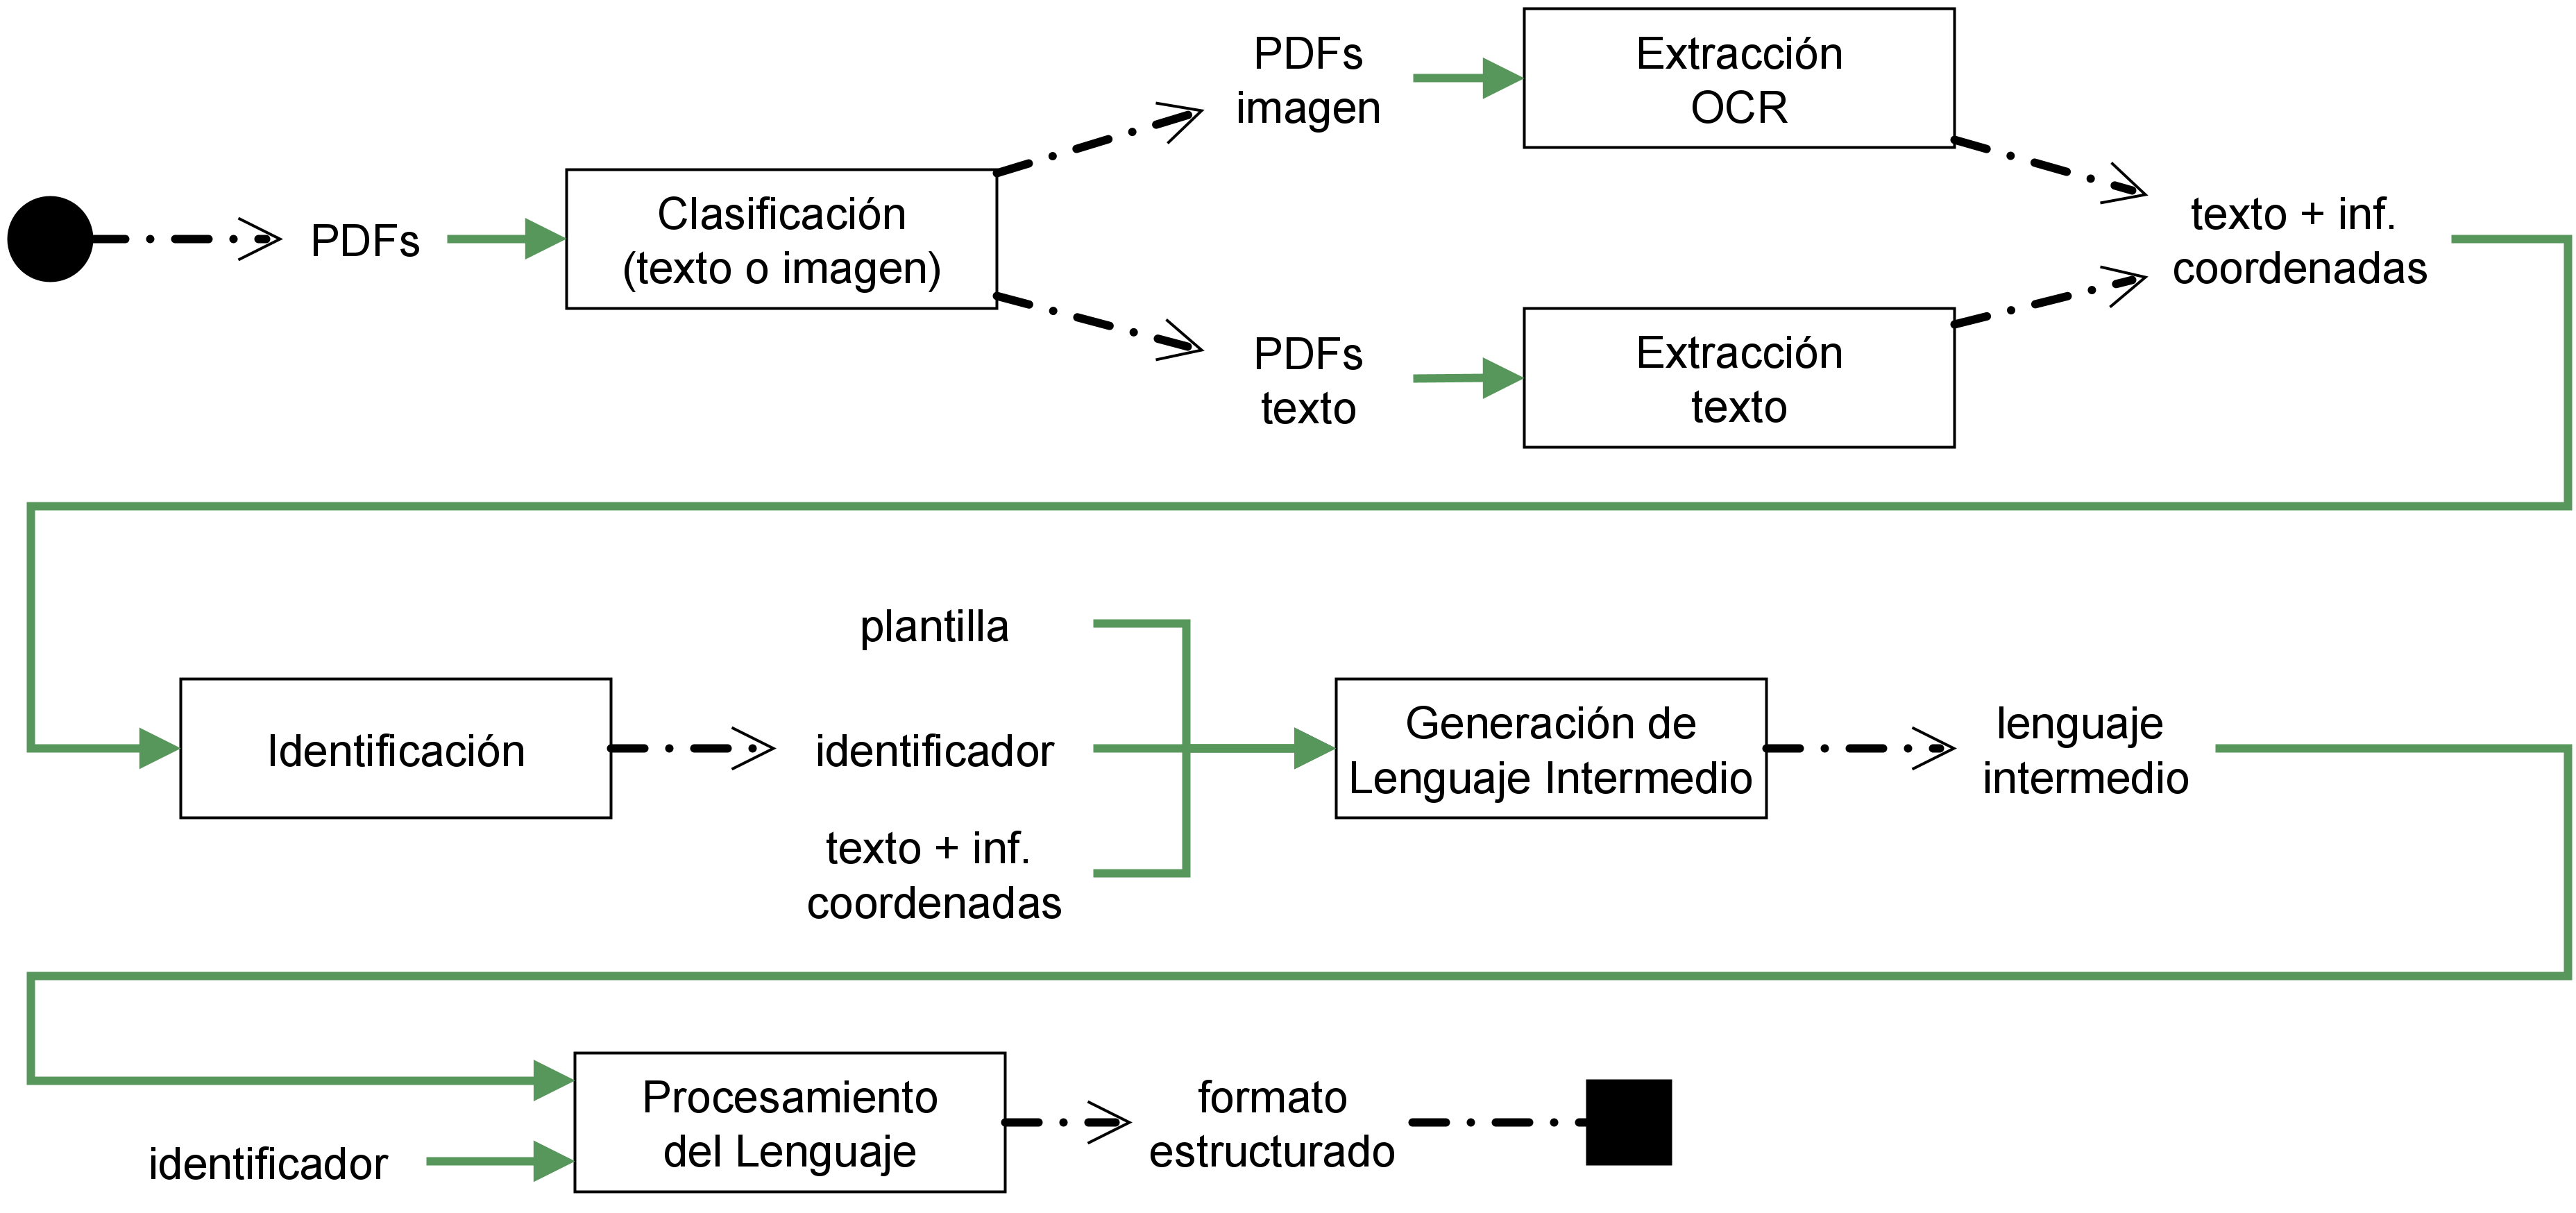
\includegraphics[width=1.0\textwidth]{imaxes/h-implementacion/vision-general-del-sistema-2}
    \caption{Visión general del pipeline del sistema}
    \label{fig:vision-general-del-sistema}
\end{figure}

El proceso comienza cuando se proporcionan al sistema un nuevo conjunto de ficheros PDF. La primera acción realiza la clasificación, según el tipo contenido de los PDF sean páginas con texto o con imágenes. El sistema mantienen el estado colocando los ficheros en las rutas apropiadas. 

A continuación se procede a la extracción de la información de los documentos. Además del propio texto, directamente visible, se genera la información de coordenadas que se utilizará para seleccionar los contenidos relevantes.

El proceso sigue con la identificación de los documentos con el objetivo de poder seleccionar la plantilla correcta, si está dada de alta en el sistema. 

Con toda la información obtenida se puede comenzar la generación del lenguaje intermedio de cada página. Para ello, la información de entrada es la plantilla, el código del identificador encontrado y el texto con las coordenadas de la etapa de extracción.

Por último se transforma el lenguaje intermedio y se genera toda la información de salida del sistema. El identificador es utilizado para seleccionar el parser necesario para tratar el documento. Todos los datos de salida son movidos a un directorio de resultados y se genera la marca de finalización del tratamiento.

De todas estas tareas se ocupa el engine del sistema, que invoca uno a uno los scripts correspondientes a cada tarea haciendo evolucionar el trabajo.

\subsection{Creación de un nuevo trabajo}

Si bien la imagen \ref{fig:vision-general-del-sistema} representa el flujo de datos a nivel general, para comenzar el tratamiento se sigue un proceso formalizado en tres pasos. 

Primero el Sistema Externo solicita un identificador para el nuevo job. En ese momento el motor genera el código y lo utiliza para crear las rutas de directorios necesarias para ubicar los resultados de cada etapa. El identificador se obtiene de la fecha UTC actual concatenando segundos y nanosegundos. Se recurre al comando \verb|date| para ello, como se muestra en \ref{lst:creacion-job-id}).

\begin{lstlisting}[language=bash,caption={Obtención del identificador de un trabajo},label=lst:creacion-job-id]
job_id=$(date -u +%s%6N)
\end{lstlisting}

Utilizando el identificador, el Sistema Externo formar el path estándar donde deberá depositar el fichero comprimido. Por último se le debe indicar al motor que comience el procesamiento del trabajo para el id deseado.

\subsection{Clasificación de los ficheros}

Como primera acción para tratar correctamente los fichero se realiza un saneamiento de los nombres. Aplicar un nombrado homogéneo evita problemas en la construcción de las rutas en el sistema de ficheros. También se descartan los directorios que el fichero comprimido facilitado pudiera contener. Los ficheros simplemente se nombran secuencialmente desde 1 y de forma creciente.

Los PDF recibidos deben ser clasificados dependiendo de su contenido. En unos casos es posible utilizar directamente el texto del documento. Para los restantes se procederá a utilizar el procedimiento OCR, como se ha explicado anteriormente. La clasificación se realiza por medio de un test de extracción de texto y se busca una respuesta positiva en la salida.

En \verb|extract-text.sh| se utiliza la herramienta \verb|pdftotext| sobre cada página de cada fichero. En \ref{lst:extraccion-text-inicial} se puede ver la instrucción utilizada.

\begin{lstlisting}[language=bash,caption={Extracción tentativa del texto},label=lst:extraccion-text-inicial]
for ((page=1; page<=$last_page; page++))
do
    page_number="$($engine_dir/fix-page-numbers.sh $page)"
    pdftotext -f $page -l $page -layout "$line" "$n-$page_number.txt"
done
\end{lstlisting}

Cuando un documento no contiene texto, el fichero de la información extraída únicamente almacena caracteres de salto de página, \verb|0x0C|, que son introducidos por el propio \verb|pdftotext|. Estos caracteres pueden ser localizados mediante un editor hexadecimal, como se muestra en \ref{lst:deteccion-salto-pagina}. Tanto si se ejecuta el cuerpo del \verb|if| como del \verb|elif| se trata de un caso de imagen y el fichero es movido al directorio para los casos de imagen.

\begin{lstlisting}[language=bash,caption={Detección del salto de página},label=lst:deteccion-salto-pagina]
if [ "$(hexdump -e '1/1 "%02X\n"' $i | tr '\n' ' ')" = '0C ' ]
then
    mv $i $base_image_dir
elif [ "$(hexdump -e '1/1 "%02X\n"' $i | tr '\n' ' ')" = '0C * ' ]
then
    mv $i $base_image_dir
fi
\end{lstlisting}

\subsection{Extracción de datos}

Previamente al proceso OCR, el script \verb|extract-images.sh| se encarga de extraer las imágenes contenidas en los ficheros seleccionados en el paso anterior. En este proceso se recupera la información original contenida en el PDF, no se trata de una \emph{foto} de la página. Se utiliza la herramienta \verb|pdfimages| con el flag \verb|-j|. Si las imágenes presentes en el PDF fueron almacenadas en formato JPEG, con este flag se conseguirá recuperar la información sin realizar transformaciones, ya que el formato PDF soporta la codificación JPEG de forma nativa por medio de los filtros DCTDecode y JPXDecode \cite[23]{adobe_book_iso32000-1}. Además, al no requerir transformación la extracción es muy rápida.

El siguiente paso obtiene la información de coordenadas de los casos de texto, nuevamente con \verb|pdftotext|. Se generan los ficheros XHTML cuando se invoca la herramienta con el flag \verb| -bbox-layout|. En \ref{lst:extraccion-text-coord} se muestra un extracto del contenido típico que luego será procesado por el generador de código intermedio. Como se puede apreciar, se identifican la palabras individuales y la línea a la que pertenecen.

\begin{lstlisting}[language=XML,caption={Extracción de texto con información de coordenadas},label=lst:extraccion-text-coord]
<flow>
    <block xMin="1594.583333" yMin="461.616667" 
            xMax="2148.275000" yMax="496.304167">
    <line xMin="1594.583333" yMin="461.616667" 
            xMax="2148.275000" yMax="496.304167">
        <word xMin="1594.583333" yMin="464.608333" xMax="1690.916667" 
                yMax="495.441667">Fecha</word>
        <word xMin="1700.183333" yMin="464.608333" xMax="1739.083333"   
                yMax="495.441667">de</word>
        <word xMin="1748.350000" yMin="464.608333" xMax="1939.116667" 
                yMax="495.441667">facturación:</word>
    </line>
</block>
\end{lstlisting}

Completada la extracción de texto se da paso al proceso de OCR. El script \verb|image-apply-ocr.sh| recorre el directorio donde están almacenadas las imágenes recuperadas. 

En la invocación de Tesseract \ref{lst:invocacion-de-tesseract} se le indican varios parámetros importantes. Debe utilizar utilizar los conjuntos de entrenamiento para el contenido en castellano (\verb|-l spa|), el número de \acrlong{ppp} se fija a 300 (\verb|--dpi 300|) ya que es un tamaño adecuado que las imágenes deben tener para que el proceso OCR tenga calidad suficiente. Tesseract dispone de varios algoritmos para interpretar el layout de documento. En este caso, al trabajar directamente con las coordenadas, no es necesario un layout y se le indica que capture la máxima información posible independientemente del orden (\verb|--psm 11|).

\begin{lstlisting}[language=XML,caption={Extracción de texto con información de coordenadas},label=lst:invocacion-de-tesseract]
tesseract $file_path "$outputbase" \
    -l spa \
    --dpi 300 \
    --psm 11 \
    -c page_separator='' \
    --tessdata-dir "$tessdata_dir" \
    $tessconfig_file
\end{lstlisting}

% TODO separación de las páginas individuales

% TODO comentar caso con pdftotext
% TODO incluir flags utilizados
% TODO ejemplo de salida de la información

% TODO comentar caso con OCR
% TODO parámetros de Tesseract
% TODO para cumplir con el requisito de tiempo reducido de ejecución se configuró Tesseract para emplear todos los cores disponibles en la máquina
% TODO ejemplo de salida de la información

\subsection{Identificación}

% TODO modelo de identificación. Explicar que está pensado para ser extensible a uso de BD u otras fuentes de información
% TODO explicar como se recorre el array en bash
% TODO mostrar la lista de identificadores
% TODO mostrar como se marca el directorio con el fichero .id

\subsection{Plantillas y regiones}
% TODO Tipos de regiones
% TODO información contenida en las plantillas (la que no se refiere a coordenadas)

\subsection{Generación del lenguaje intermedio}
% TODO describir la implementación en etapas, como el diagrama general
    % TODO Concepto de línea de identificación
    % TODO Asignación de palabras a regiones
    % TODO información de bounding box
% TODO mostrar el código intermedio
% TODO introducir el problema de indentificar las líneas
% TODO explicar se utiliza el algoritmo de Hough en los ejemplos donde es efectivo
% TODO explicar mejora en el algoritmo para asignación de palabras a regiones para cumplir con el requisito no funcionar de mantener los tiempos contenidos

\subsection{Procesamiento del lenguaje intermedio}
% TODO explicar como es la estructura general de Flex / Bison
% TODO mostrar las modificaciones introducidas
% TODO explicar la carga dinámica de librerías
% TODO Mencionar que el modelo de plugins permite entregar al cliente solo los modelos comprados
% TODO mostrar como es el formato de un fichero Flex y también Bison
% TODO Mostrar como se utiliza la librería para generación de ficheros JSON
% TODO Mencionar el pretty printing con jq
% TODO explicar como es el flujo de información y por qué los terminales y no terminales llevan un tipo de dato en Bison

\subsection{Un engine modular}
% TODO Detalle de la estructura de directorios considerada
% TODO Se imita un modelo de procesamiento en batch
% TODO Se generan códigos de identificación de los jobs recibidos. También marca final.

El motor del sistema es el componente implementado en Bash. Esta decisión se tomó para facilitar el manejo de los ficheros dentro de la estructura de directorios. Además se utilizan herramientas en la consola, que sería más engorroso utilizar desde otros lenguajes de programación.

\section{Compilación y despliegue}

\subsection{Makefile}
% TODO mostrar el Makefile

\subsection{Ansible}
% TODO mostrar script Ansible

\subsection{Docker}
% TODO Mostrar fichero de configuración Docker y su uso

% TODO valorar si incluir capítulo o sección de pruebas. O, al menos, de pruebas realizadas.

\section{Editor de coordenadas}

